\section{Prototype}
\chapterauthor{Agnieszka Kuleta} \newline
Having prepared principal requirements we wanted to validate  them  and make sure whether we have include everything we needed to make our system work. To do it, we have chosen the  technique of validation called prototyping. This simplified model  helped us to detect usability errors earlier and correct them not only on lower cost, but also it was more time efficient. Our prototype was design as a Hi-Fi prototype using \textbf{Figma} environment and it can be accessed \href{https://www.figma.com/design/ypRomVQ6laijnORYDQrsFE/Prototype_bachellor_final?node-id=0-1&t=8WDgKX0NAGXPXQpk-1}{here}. It is  working and interactive, so it was perfect  to present it to our stakeholders and demonstrate how are software would look like and which usability features it will include. 
Moreover, we wanted to make sure that the design of our system will ensure pleasure user-experience. To achieve that we focused on the  following features:
\begin{itemize}
    \item \textbf{Readable text}
    \item \textbf{A large number of images}, to enhance recognizability over text
    \item \textbf{Numerous icons}, that are functional and visually distinctive
    \item \textbf{Bright, well-matched colors}, that are engaging without being overwhelming
\end{itemize}

We have tried our portal to look simple and elegant, we did it by making it visually consistent and standardize. Moreover, we have prepared navigation like bottoms, flags and labels.

\begin{figure}[h]
    \centering
    % Row 1
    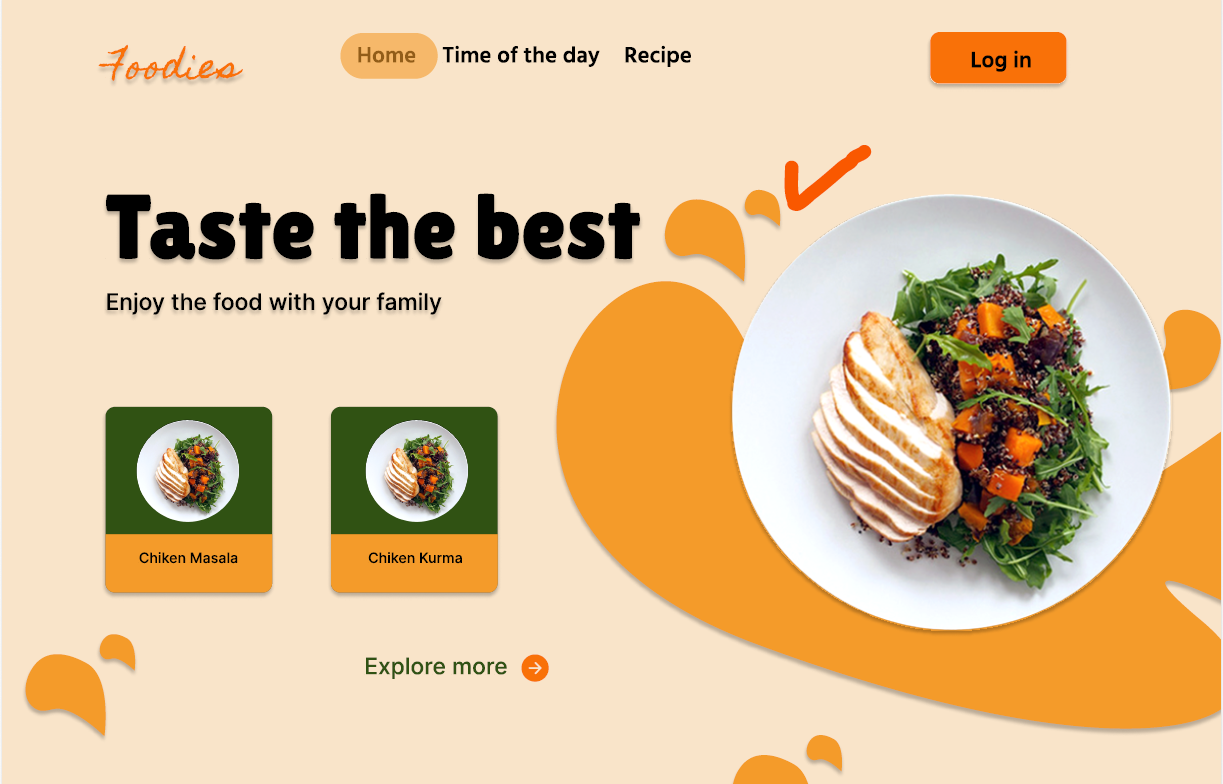
\includegraphics[width=0.45\textwidth]{images/Prototype/screen1.png} % First image
    \hfill
    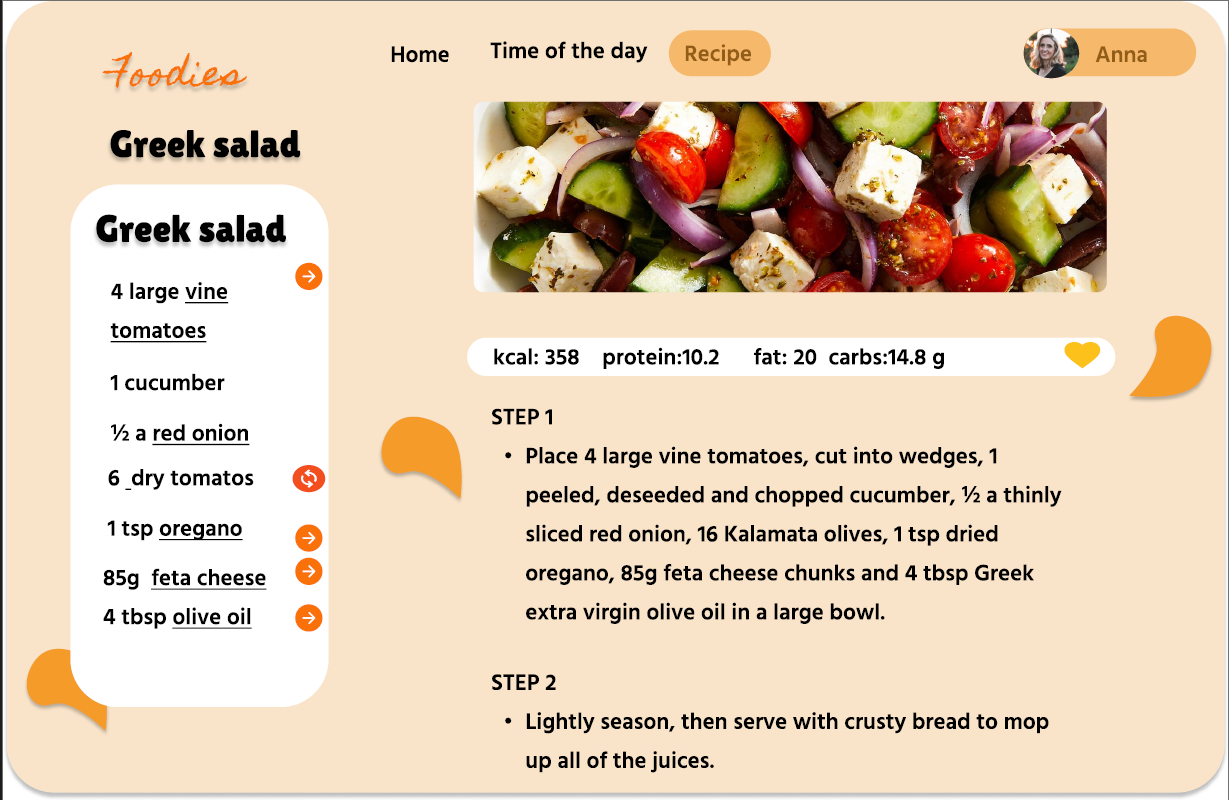
\includegraphics[width=0.45\textwidth]{images/Prototype/screen2.png} % Second image
    \vspace{0.5cm} % Space between rows

    % Row 2
    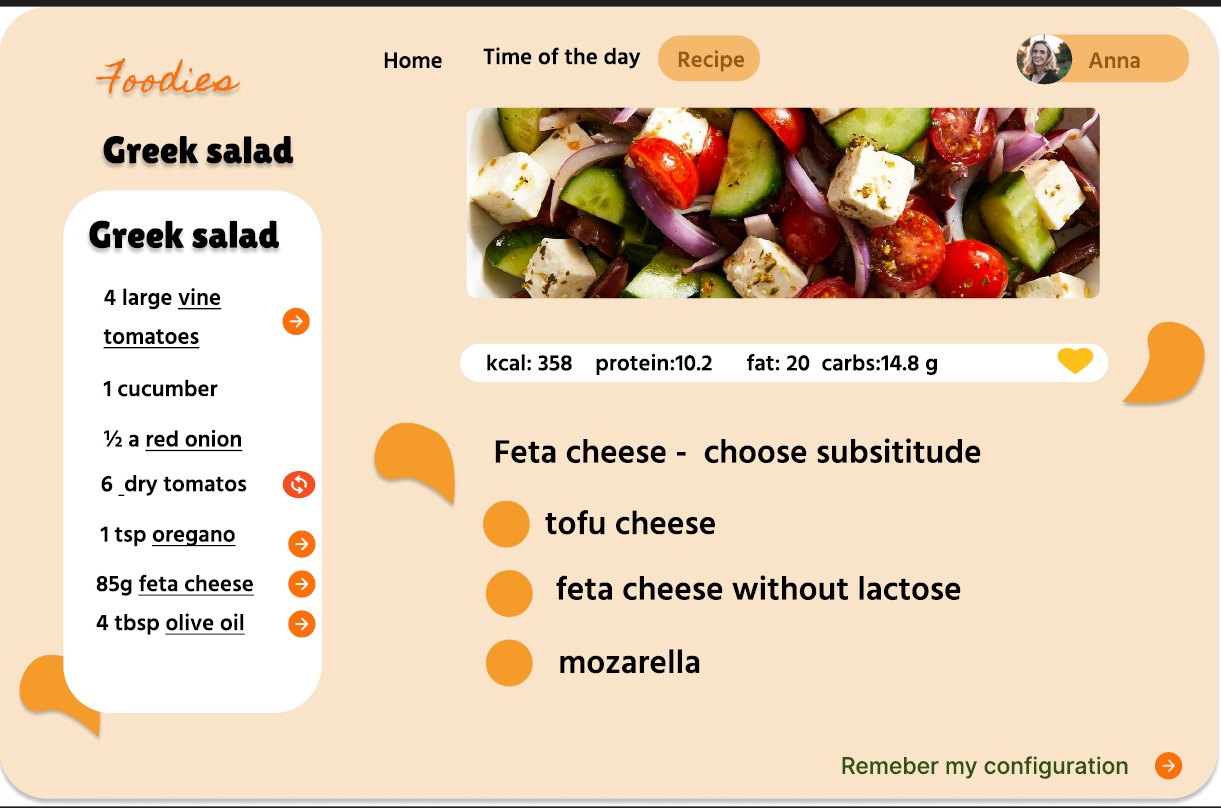
\includegraphics[width=0.45\textwidth]{images/Prototype/screen3.png} % Third image
    \hfill
    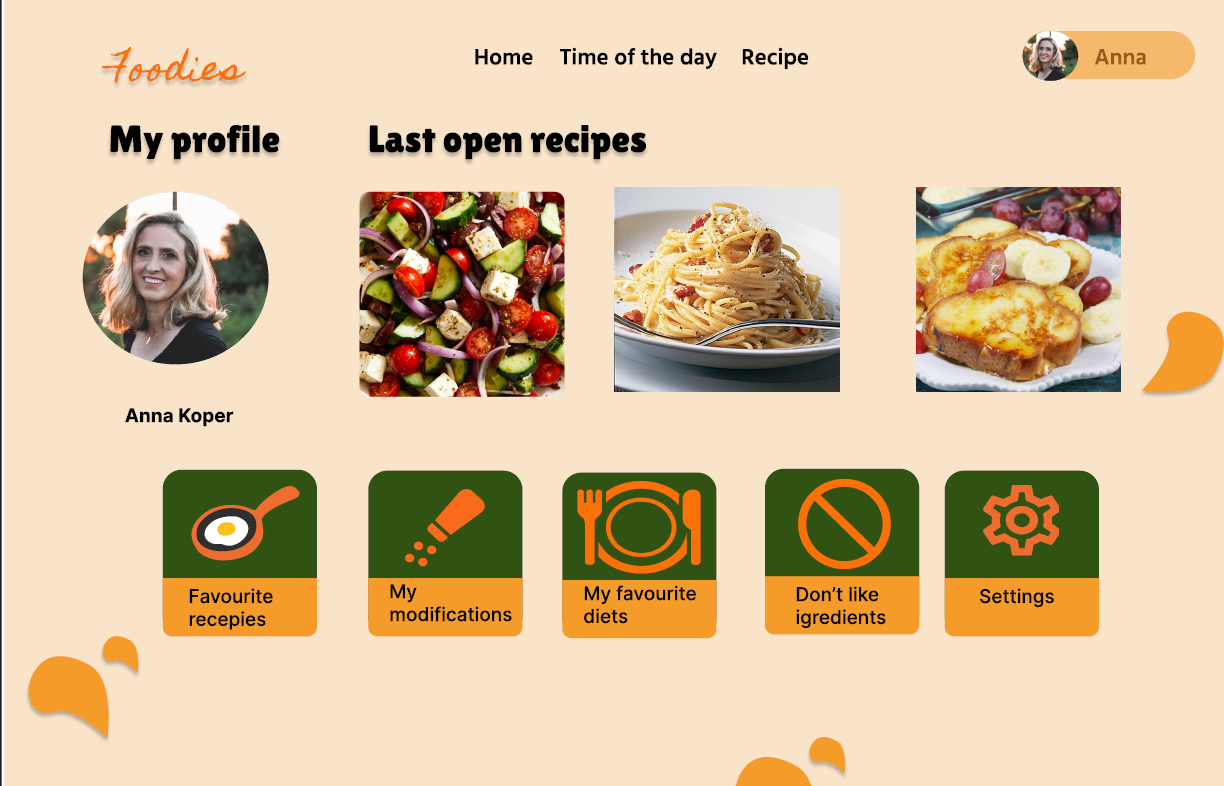
\includegraphics[width=0.45\textwidth]{images/Prototype/screen4.png} % Fourth image

    \caption{Four prototype screens arranged in a 2x2 layout.}
    \label{fig:four_images}
\end{figure}

Finally, when we got our vision of design and all requirements verified and gathered we started to build the architecture of our system which will be described in the next section of the chapter.

\section{Application Architecture}
\chapterauthor{Wiktor Czetyrbok}


\subsection{Backend Service: Java Spring Boot}\label{subsec:Backend Service: Java Spring Boot}

For the backend of our application, we decided to use Spring Boot, it is a robust framework that provides an efficient way to implement a scalable, modular architecture using the MVC (Model-View-Controller) design pattern. Spring Boot is particularly well-suited for building RESTful APIs, which are the base of communication in a microservices-based architecture. 

Spring Boot simplifies the creation of RESTful web services by using its built-in support for Spring Web. REST controllers manage incoming requests, route them to the appropriate service layer, and return responses in standard formats like JSON. Figure \ref{fig:restController} shows an example of a REST API controller from culinary-user-application (backend service), which shows how to handle common HTTP methods such as GET and PUT.
\renewcommand\theFancyVerbLine{\large\arabic{FancyVerbLine}}
{
\begin{minted}[linenos, frame=single]{java}
@RestController
@RequestMapping(path = "/api/user")
public class UserController {
    private final UserService userService;

    @GetMapping("/username/{userName}")
    public UserDetailsDTO getUserByUserName(@PathVariable String userName) {
        return userService.getUserByUserName(userName);
    }

    @PutMapping("/{userId}")
    public UserDetailsDTO updateUser(@PathVariable long userId, 
    @RequestBody PutUserDTO putUserDTO) {
        return userService.updateUser(userId, putUserDTO);
    }
}
\end{minted}
\captionof{figure}{Example of REST controller in culinary-user-service}
\label{fig:restController}
}

The Spring Boot annotations in the code simplify the creation of RESTful web services. The \texttt{@RestController} annotation indentifies the class as a REST controller, where the return values of the methods are automatically serialized into JSON and included in the response body. \texttt{@RequestMapping(path = "/api/user")} maps HTTP requests that match the specified path \texttt{(/api/user)} to this controller. The \texttt{@GetMapping("/username/{userName}")} annotation maps HTTP GET requests to the method, with \texttt{{userName}} representing a dynamic path variable passed to the method. \texttt{@PathVariable} binds the method parameter to the path variable from the URL. The \texttt{@PutMapping("/{userId}")} annotation maps HTTP PUT requests to the method, with {userId} as a dynamic path variable. Finally, \texttt{@RequestBody} tells Spring to deserialize the HTTP request body into a specified Java object, in this case, \texttt{PutUserDTO}.  With this standardized use of annotations, it becomes quick and easy to create a set of APIs, without the complexity of manually handling HTTP request structures.


Spring Boot implements the Model-View-Controller paradigm to organize code effectively. This pattern helps to divide code into distinct layers, each of which carries out a specific set of tasks as shown in the Figure \ref{fig:mvc}).
 \begin{figure}[H]
    \centering
    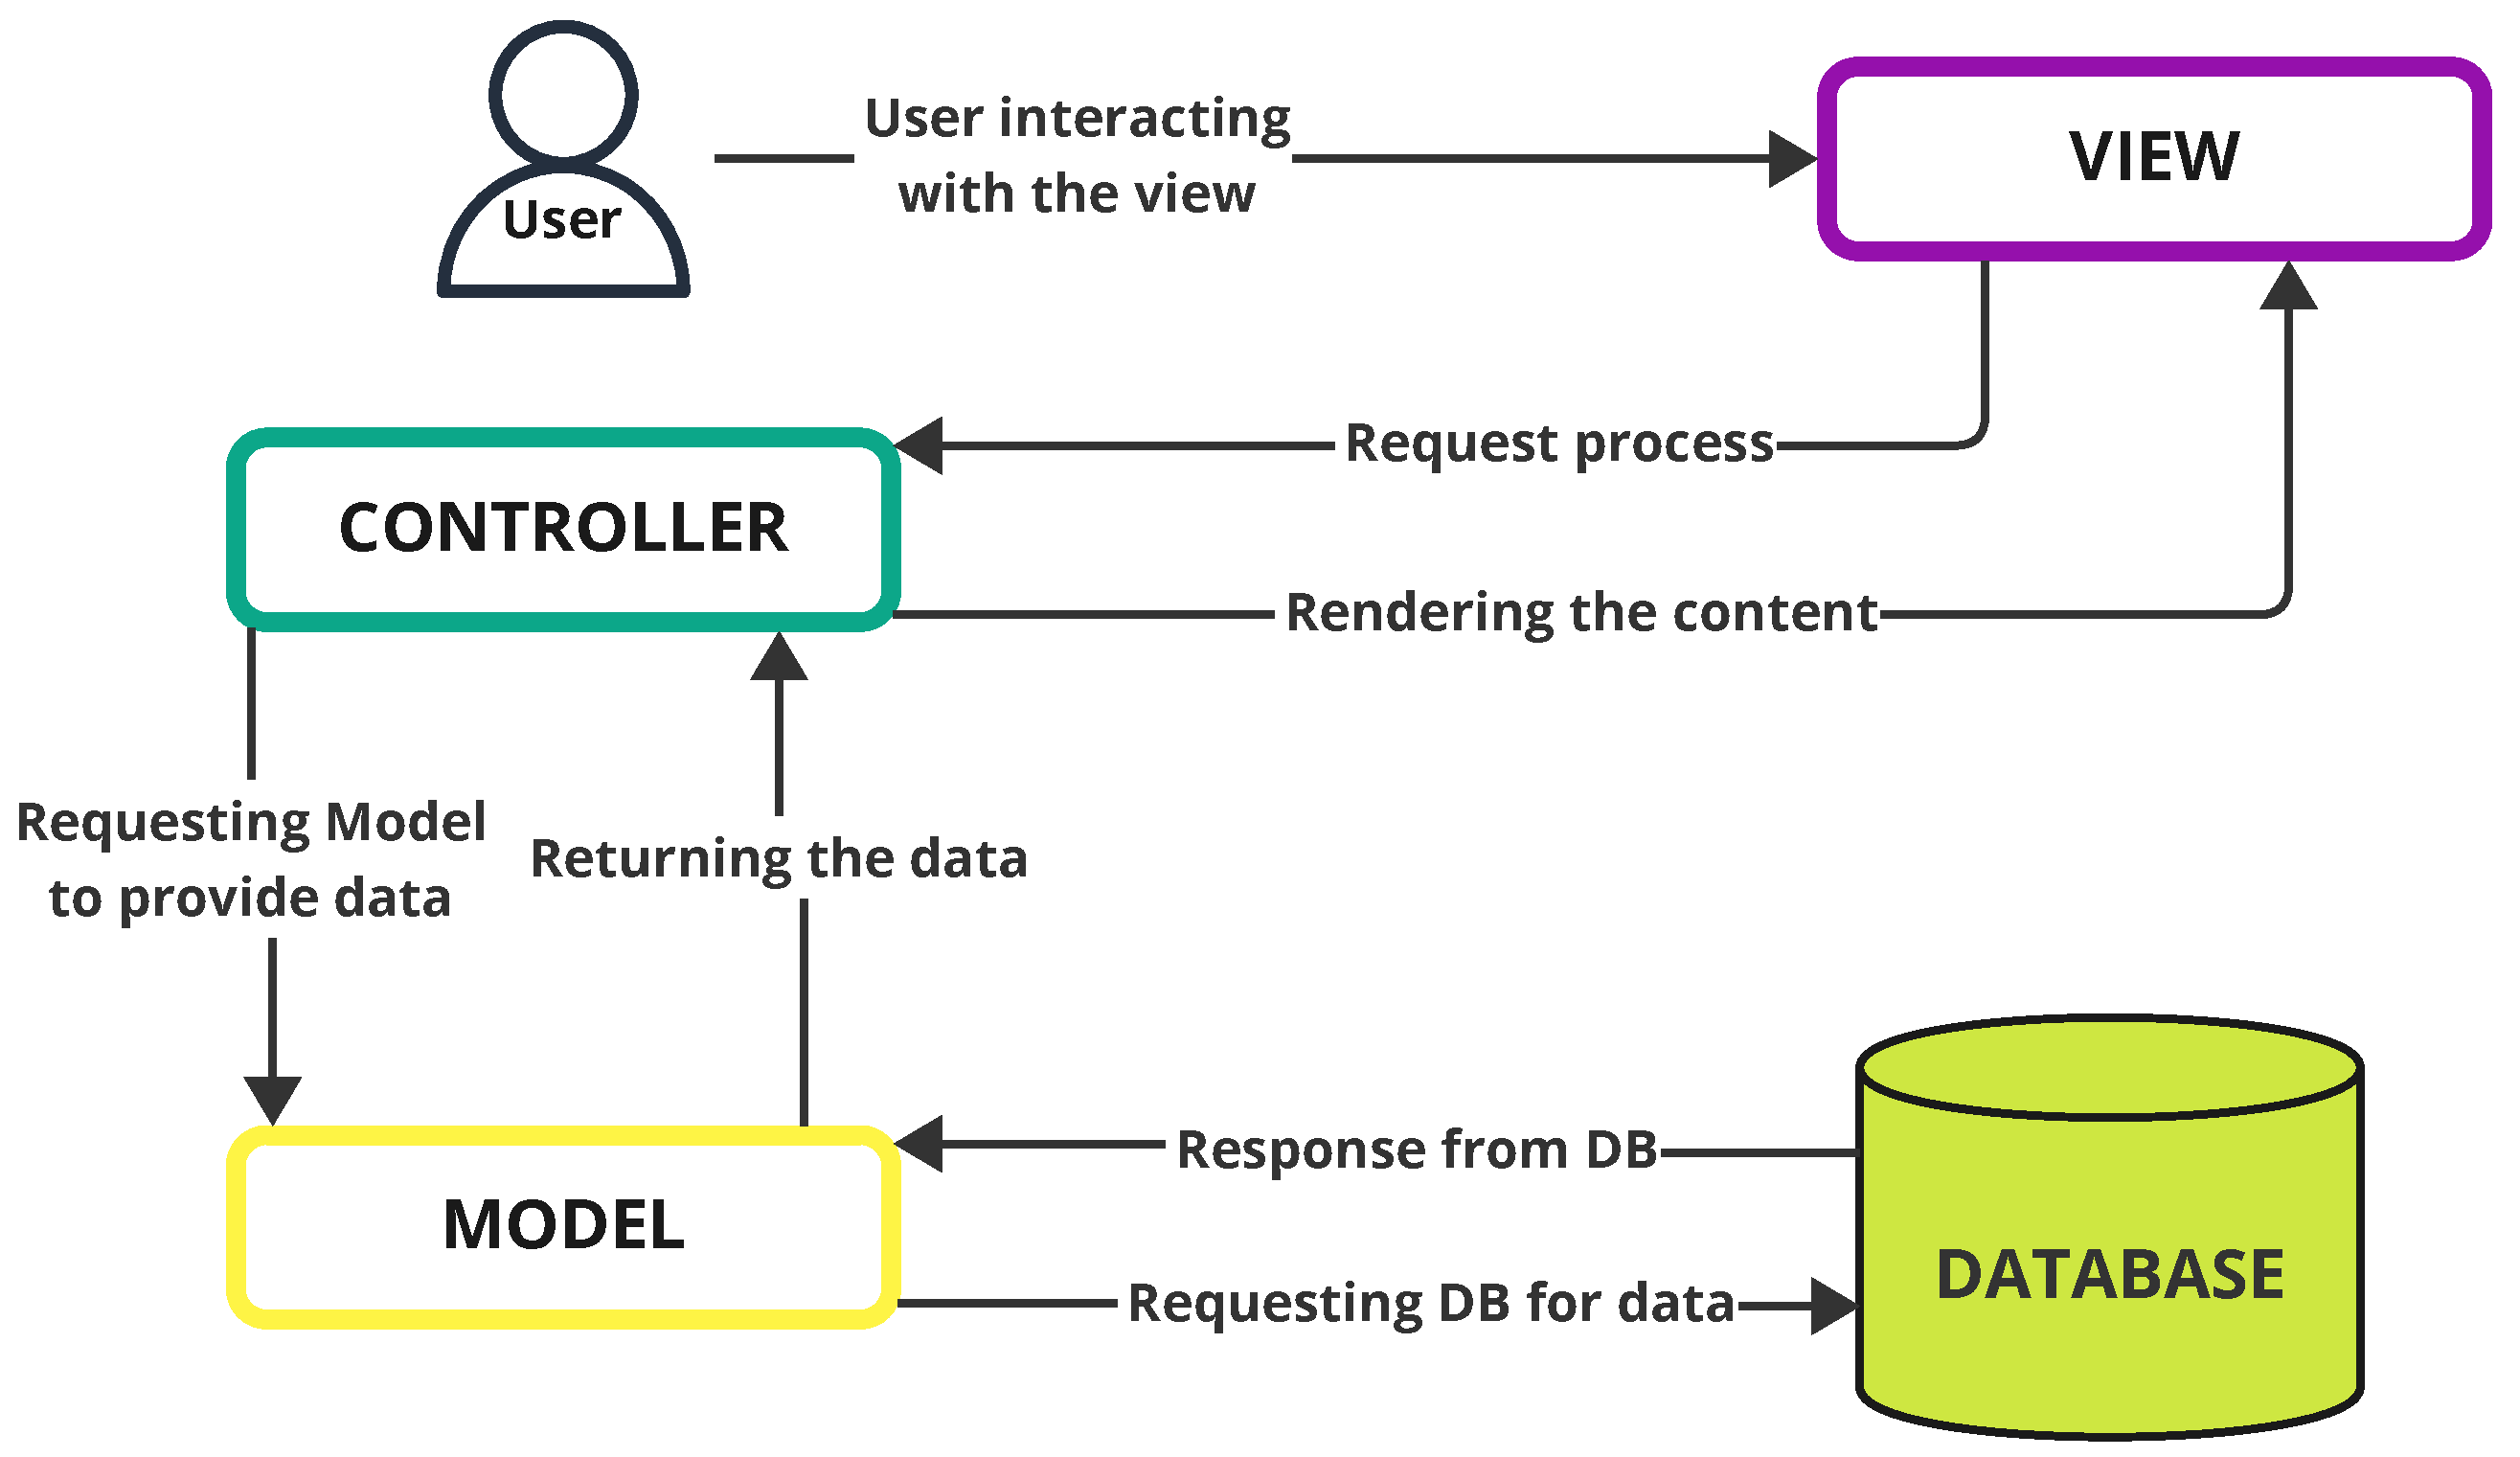
\includegraphics[width=0.8\textwidth]{images/mvc.pdf}
    \caption{ Model View Controller design pattern visualization (created by the Authors)}
    \label{fig:mvc}
\end{figure}
While we have already described the Controller in Spring Boot, the Model and View components are crucial in maintaining this separation of concerns.  

The Model in Spring Boot represents the data and the business logic of the application. It typically consists of Java classes that represent entities, such as users or orders, and contain properties, along with methods to manipulate and process the data. The Model is responsible for encapsulating the application's state and handling the logic required to access and update that state. For example, a User class might contain properties such as userName, email, and password, along with getter and setter methods to manage those values. The Model can also interact with the database through repositories and services to persist and retrieve data.

The View is typically represented as HTML page in web browser, in this architecture it is interpreted as the JSON responses returned by the Spring Boot backend. These JSON responses are later consumed by the Angular frontend, which renders the data in the browser, as described in chapter \ref{subsec:Frontend: Angular}.

As the service grows, it becomes increasingly challenging to manage and document all the endpoints and DTOs (Data Transfer Objects) used in the application. This is where the Swagger tool comes in handy. Swagger, also known as OpenAPI \cite{openapi-documentation}, provides an intuitive interface for automatically documenting and visualizing REST APIs. Swagger helps by listing all available endpoints, their HTTP methods, request/response formats, and associated DTOs, making it easy to understand and test the API. The interactive UI (Fig. \ref{fig:swagger-ui}) enables developers and stakeholders to explore the API, test endpoints, and ensure consistency without relying on external tools. We implemented this in our backend service, as it exposes over 30 endpoints and multiple DTOs.
 \begin{figure}[H]
    \centering
    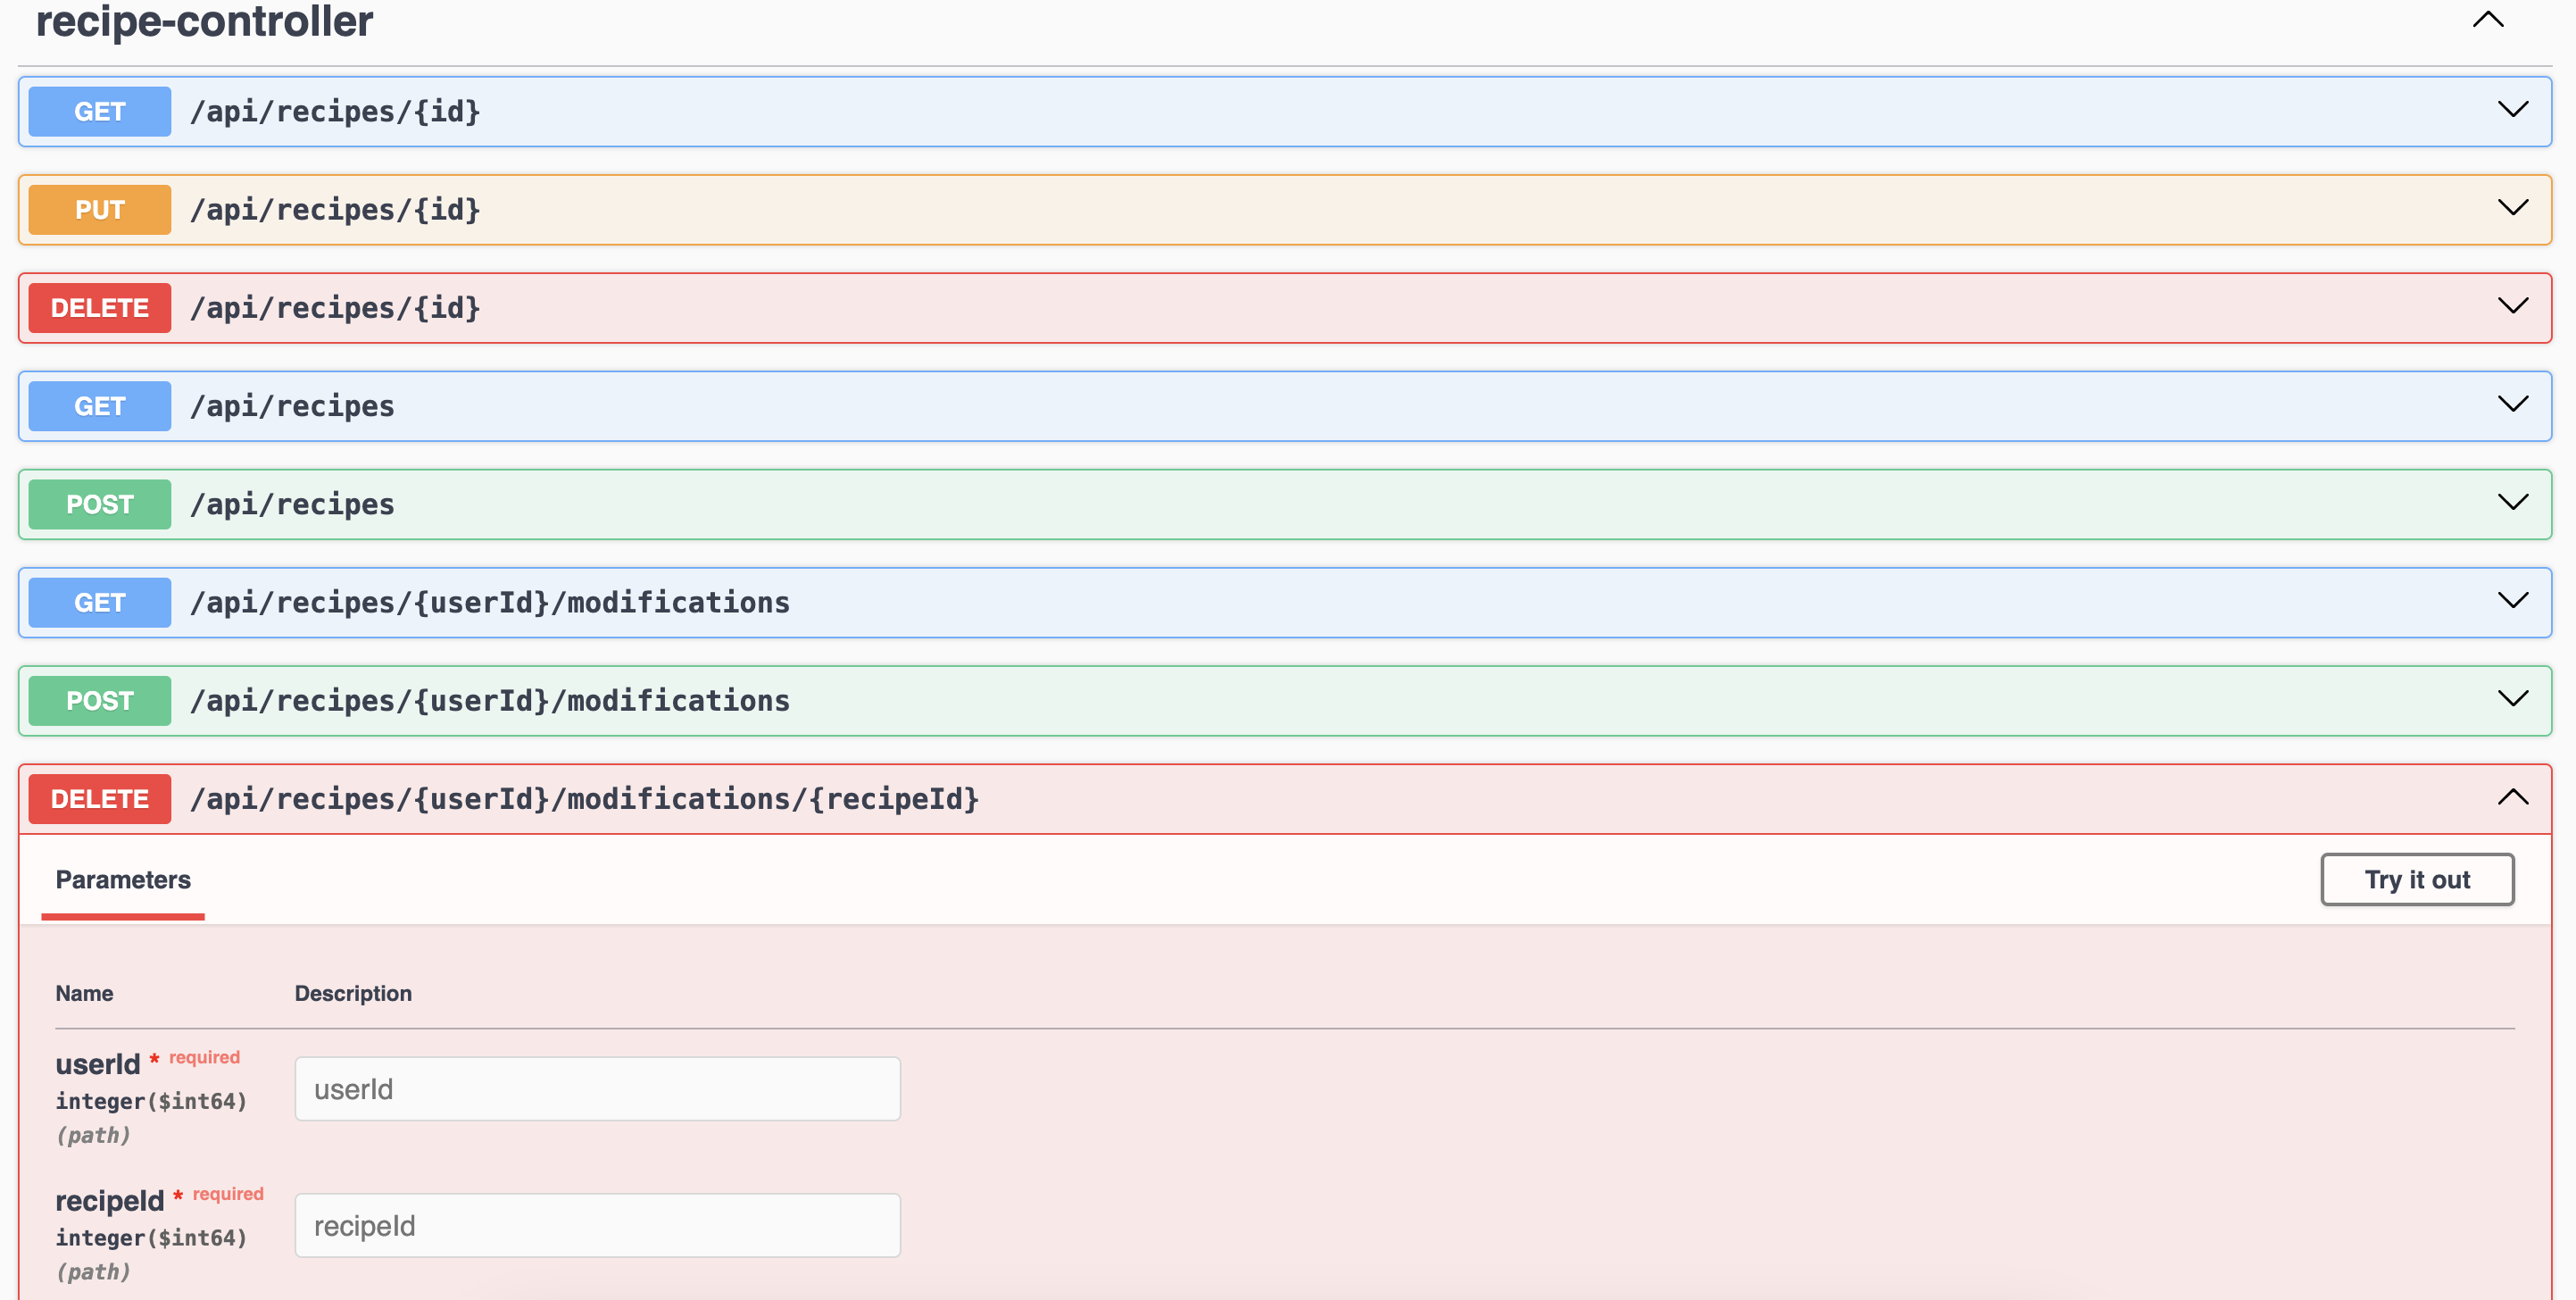
\includegraphics[width=1\textwidth]{images/swagger-ui.png}
    \caption{ OpenAPI Swagger interface for recipe-controller in culinary-user-service}
    \label{fig:swagger-ui}
\end{figure}

\subsection{Frontend: Angular}\label{subsec:Frontend: Angular}
Angular \cite{angular-documentation} is a platform and framework for building single-page applications (SPAs) using HTML and TypeScript. In the culinary-frontend-service, Angular is used to create an interactive user interface that communicates with the backend through REST API calls. The HTTPClient module in Angular simplifies making API requests to endpoints provided by the culinary-user-service, supporting data exchange for operations like user authentication, user management, retrieving recipes and other business data.

Angular’s component-based structure ensures modular, reusable UI elements, which makes the application scalable and maintainable as it grows. Additionally, Angular’s RxJS (Reactive extensions library for JavaScript) \cite{RxJS} integration efficiently manages asynchronous API responses and application state, making the frontend responsive.

Moreover, one of the key advantages of using Angular is its two-way data binding. This feature keeps the UI in sync with updates from the backend in real time, resulting in a dynamic and engaging user experience. As shown in Figure  \ref{fig:two-way-data-binding}, any change made in the view is immediately reflected in the model, and any update in the model is sent to the view. Since the view is simply a representation of the model, the controller is separated from the view.

 \begin{figure}[H]
    \centering
    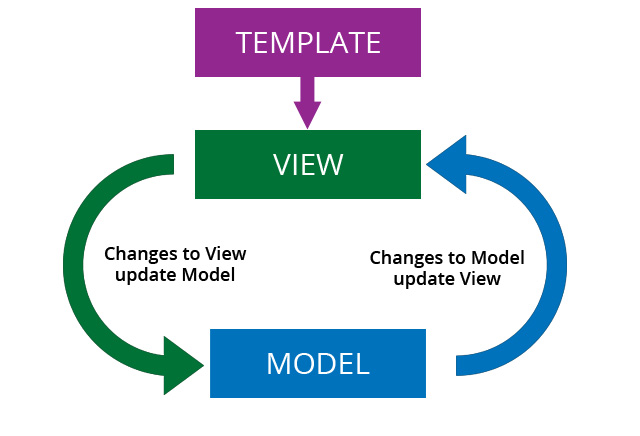
\includegraphics[width=0.6\textwidth]{images/2wouW.jpg}
    \caption{Two-way data binding [source: stackoverflow.com/questions/13504906/what-is-two-way-binding]}
    \label{fig:two-way-data-binding}
\end{figure}

To improve the design and styling of the frontend, we decided to use Tailwind CSS. Tailwind’s utility-first approach which means that it allows for highly customizable, responsive layouts without the need for writing custom CSS for every component. This helps speed up the development process, ensuring that the frontend not only looks polished but also remains flexible and adaptable to future changes. Tailwind’s classes can be easily applied to components, allowing for quick adjustments to the UI with minimal effort, while maintaining a consistent design system across the application.

\subsection{Data Layer with Java Persistence API: PostgreSQL}

Java Persistence API (JPA) \cite{jpa-documentation} is an Object-Relational Mapping (ORM) tool for the data layer in our application, enabling interaction with a relational database like PostgreSQL. JPA abstracts database operations by mapping Java objects to database tables, eliminating the need to write boilerplate SQL code. This simplifies data management, ensures consistency, and increases developer productivity. 

During local development, we also use H2 DB, it is an in-memory database that integrates with JPA. H2 allows rapid prototyping and testing without the overhead of setting up all the environment that comes when creating new database. Because we use JPA mappings switching between H2 and PostgreSQL is very straightforward, without any code changes it allows to test the app logic, achieved by only changing the database configuration in the application properties. This setup mirrors the structure of the PostgreSQL database, ensuring that development environments are closely aligned with the production. 

In JPA, entities are Java classes that represent database tables Figure \ref{fig:jpa-table}.

\clearpage % Move the figure and everything after it to a new page

{
\begin{minted}[linenos, frame=single]{java}
@Table(name = "users") // specifies SQL table name
@Entity // Maps class to a database table
public class User implements Serializable {
    @Id // marks as primary key
    @GeneratedValue(strategy = GenerationType.IDENTITY) // auto-generates id
    @Column(name = "user_id") // maps to specific column
    private Long id;
    @Column(name = "user_name")
    private String userName;
    @Column(nullable = false) // ensures that field is not null
    private String password;
}
\end{minted}
\captionof{figure}{Example of JPA Table}
\label{fig:jpa-table}
}

JPA simplifies relationships between entities, such as a one-to-many association between a User and Role, by using specific annotations, as shown on Figure \ref{fig:jpa-mapping}.
{
\begin{minted}[linenos, frame=single]{java}
@OneToMany(mappedBy = "user")
private Set<Role> roles = new HashSet<>();
\end{minted}
\captionof{figure}{One-to-many JPA mapping}
\label{fig:jpa-mapping}
}

After configuring all the relationships and mappings for our database entities, we can use Spring Data JPA to interact with the database through repository interfaces. By extending JpaRepository interface, we gain access to a set of predefined methods for common operations such as saving, updating, and retrieving records, without needing to implement them ourselves. This eliminates the need to write boilerplate code for queries. JPA allows us to define custom queries using a syntax similar to SQL. Figure \ref{fig:jpa-repository} demonstrates how to create a repository for the User entity, including a custom query to search for usernames (line 3-5) using a regular expression and predefined query to find a user by email. The findByEmail (line 7) method is automatically implemented by JPA, as long as the naming convention is followed and the correct parameter is provided. 

{
\begin{minted}[linenos, frame=single]{java}
public interface UserRepository extends JpaRepository<User, Long> {

    @Query("SELECT c FROM User c WHERE LOWER(c.userName)" +
            " LIKE LOWER(CONCAT('%', :userName, '%'))")
    Optional<User> findByUserNameRegex(@Param("userName") String userName);
    
    Optional<User> findByEmail(String email);
}
\end{minted}
\captionof{figure}{JPA repository interface}
\label{fig:jpa-repository}
}
\subsection{User session management: Redis}

Redis \cite{redis} is an in-memory key-value database that is widely used for caching or session management. Making it an excellent choice for storing user sessions in the culinary-user-service application. By leveraging Redis, the application benefits from enhanced performance, scalability, and reliability. Performance is a key advantage of Redis, as it stores data in memory, enabling extremely fast read and write operations, which is essential for session management. Redis is also highly scalable, capable of handling a large number of read and write operations per second, making it ideal for high-traffic applications. Furthermore, Redis can be scaled horizontally by adding additional nodes to the cluster, supporting the growth of the application. Another significant feature of Redis is its support for data persistence, which allows session data to be saved to disk and restored in the event of a server restart, ensuring that user sessions are not lost during a failure. Additionally, Redis integrates well with Spring Boot, simplifying its setup and use for session management. Spring Session, for example, provides robust support for managing user sessions in a distributed environment using Redis, enabling consistent and reliable session handling across multiple instances of the application.

Redis was configured in backend application by using \textit{spring-boot-starter-data-redis} package. Figure \ref{fig:RedisConfig} illustrates the configuration class used to establish the Redis connection and enable session database integration within the backend application.
\renewcommand\theFancyVerbLine{\large\arabic{FancyVerbLine}}
{
\begin{minted}[linenos, frame=single]{java}
@Configuration
// Enables Redis for managing Spring session data.
@EnableRedisIndexedHttpSession  
@RequiredArgsConstructor
 // Activates this configuration only in non-local and non-test profiles.
@Profile({"!local & !test"})
public class RedisConfig extends AbstractHttpSessionApplicationInitializer {

    // Connection properties, injected from the application's configuration file
    private final RedisProperties redisProperties;

    @Bean
    public LettuceConnectionFactory connectionFactory() {
        RedisStandaloneConfiguration configuration =
                new RedisStandaloneConfiguration(this.redisProperties.getHost(),
                    this.redisProperties.getPort());
        configuration.setPassword(redisProperties.getPassword());
        // Returns a factory for creating connections to Redis.
        return new LettuceConnectionFactory(configuration);
    }

}
\end{minted}
\captionof{figure}{Configuration class for Redis connections and sessions}
\label{fig:RedisConfig}
}


Configuration for Redis-Backed session management in a Spring properties is defined in application.yaml file, Figure \ref{fig:app.props}).

\renewcommand\theFancyVerbLine{\large\arabic{FancyVerbLine}}
{
\begin{minted}[linenos, frame=single]{yaml}
server:
  servlet:
    session:
      cookie:
        domain: localhost # session cookie domain for local development.
        http-only: true # not accessible via JavaScript
        max-age: 600 # max age of the session cookie
        name: JSESSIONID # cookie name to track the session.
        path: / # path where cookie is valid, set to the root
        # blocks the browser from sending the cookie with cross-site requests
        same-site: strict 
      timeout: 1m # session timeout duration
      tracking-modes: cookie # cookies are used to track the session
\end{minted}
\captionof{figure}{Session management configuration properties}
\label{fig:app.props}
}

We set up configuration classes for local Redis connection and session database integration in development and test environments. In local/test versions we create Redis instance in applications runtime, as shown on Figure \ref{fig:redisServer}.

{
\begin{minted}[linenos, frame=single]{java}
@Configuration
@Profile({"local", "test"})
public class RedisConfig {

    private final RedisServer redisServer;

    public RedisConfig() throws IOException {
        this.redisServer = new RedisServer(6379);
    }

    @PostConstruct
    public void postConstruct() throws IOException {
        redisServer.start();
    }

    @PreDestroy
    public void preDestroy() throws IOException {
        redisServer.stop();
    }
}
\end{minted}
\captionof{figure}{In memory Redis database configuration}
\label{fig:redisServer}
}



After runtime database is created, we can connect to it and enable Redis repositories by providing DB host as localhost and appropriate port defined before, as can be seen in Figure \ref{fig:EnablingRedisRepositories}. 
{
\begin{minted}[linenos, frame=single]{java}
@Configuration
@EnableRedisRepositories
@Profile({"local", "test"})
public class LocalBeanConfig {

    @Bean
    public LettuceConnectionFactory redisConnectionFactory() {
        return new LettuceConnectionFactory("localhost", 6379);
    }

    @Bean
    public RedisTemplate<?, ?> redisTemplate(
    LettuceConnectionFactory connectionFactory) {
        RedisTemplate<byte[], byte[]> template = new RedisTemplate<>();
        template.setConnectionFactory(connectionFactory);
        return template;
    }
}
\end{minted}
\captionof{figure}{Enabling Redis Repositories}
\label{fig:EnablingRedisRepositories}
}
\subsection{Containerization: Docker}

Containerization \cite{containers} is a software deployment technology that packages an application and all its dependencies (e.g., libraries, configuration files) into a single lightweight, portable unit called a container. These containers can run consistently across different computing environments, such as development and production. When first introduced, containerization was revolutionary because it allowed engineers to streamline the development process by eliminating the need to set up complex dependencies, libraries, environments, and manage virtual machine images.

To implement it in our services, we decided to use Docker platform. Docker is a platform that allows you to "build, ship, and run any app, anywhere." It has come a long way in an incredibly short time and is now considered a standard way of solving one of the most expensive aspects of software: deployment, as noted by Ian Miell and Aidan Hobson S. \cite{Docker}.

In our case, containerization also streamlined the deployment process by creating a local development environment that closely mimics the cloud environment. Using Docker, we hosted essential services such as databases in containers, ensuring consistency across environments. By using docker-compose, we could define the multi-container setups with ease.

Figure \ref{fig:docker-compose} demonstrates how instances for PostgreSQL and Redis are configured with Docker in our local environment, mimicking the cloud based one. Specific ports have to be exposed, and environment variables are set to manage database credentials and other settings. With Docker running in the background, executing the command docker-compose up initializes the services automatically, downloading the required images from an online repository if not already available locally.
{
\begin{minted}[linenos, frame=single]{yaml}
version: '3.9'
services:
  db:
    image: postgres:latest
    ports:
      - "5432:5432"
    restart: always
    environment:
      POSTGRES_DB: culinary
      POSTGRES_USER: postgres
      POSTGRES_PASSWORD: postgres

  redis:
    image: redis:alpine
    container_name: redis
    ports:
      - "6379:6379"
    environment:
      REDIS_HOST: localhost
      REDIS_PASSWORD: session
\end{minted}
\captionof{figure}{Docker compose file for setting up the databases}
\label{fig:docker-compose}
}
The cloud hosting engine discussed in Section \ref{subsec:Google App Engine Flex} uses images specified by Dockerfiles for both the backend and frontend services. Dockerfiles are essentially sets of instructions for creating an image of the application. For the Angular frontend service, we have defined the Dockerfile, displayed on Figure \ref{fig:Dockerfile}.
{
\begin{minted}[linenos, frame=single]{Dockerfile}
FROM node:14 AS build
WORKDIR /app
COPY package*.json ./
RUN npm install
COPY . .
RUN npm run build

FROM nginx:alpine
COPY --from=build /app/dist/culinary-frontend-service /usr/share/nginx/html
COPY nginx.conf /etc/nginx/conf.d/default.conf
EXPOSE 8080
CMD ["nginx", "-g", "daemon off;"]
\end{minted}
\captionof{figure}{Dockerfile for Angular frontend service}
\label{fig:Dockerfile}
} 

In this Dockerfile, we first specify a base image using \texttt{FROM~node:14~AS~build}, which leverages Node.js version 14 for the build process. The working directory is then set to \texttt{WORKDIR~/app}, where next operations will be done. The command \texttt{COPY~package*.json~./} ensures that the \texttt{package.json} and \texttt{package-lock.json} files, which contain all needed libraries, are copied to the container for dependency management. Next, the command \texttt{RUN~npm~install} installs all necessary dependencies, followed by \texttt{COPY~.~.}, which copies the remaining project files into the container. The build process is then executed with \texttt{RUN~npm~run~build}, producing the production-ready files in the \texttt{dist/} directory.

After the building stage, we switch to the Nginx \cite{Nginx} base image by using \texttt{FROM nginx:alpine}, a popular, lightweight, and optimized server for serving files. The command \texttt{COPY~---from=build~/app/dist/culinary-frontend-service~/usr/share/nginx/html} moves the built files from the first stage to Nginx's default HTML directory. We then include a custom Nginx configuration using \texttt{COPY~nginx.conf~/etc/nginx/conf.d/default.conf}, where the Nginx properties are set up. The command \texttt{EXPOSE 8080} declares that the container will listen for requests on port 8080, which is the default port used by Google App Engine Flex (section \ref{subsec:Google App Engine Flex}). Finally, the command \texttt{CMD["nginx","-g","daemon~off;"]} starts the Nginx server, allowing the container to stay active.


\section{Cloud Infrastructure and Deployment} 
\chapterauthor{Wiktor Czetyrbok}

This chapter outlines the components of the cloud infrastructure used in this project and details the deployment process. It describes the integration of various Google Cloud services and explains how they facilitate the development, deployment, and scaling of the application. To deploy services, establish secure and efficient communication between components, and connect to the database, the project leverages multiple cloud services. These services, hosted by third-party providers, function as infrastructure, platforms, or software that support the developers.

\subsection{Google App Engine Flex}\label{subsec:Google App Engine Flex}

Google App Engine (GAE) Flexible Environment \cite{GAE} is an excellent platform for deploying modern, containerized applications like culinary-user-service (backend in Spring) and culinary-frontend-service (frontend). Unlike the standard environment, GAE Flex offers greater flexibility by supporting Docker-based deployment, allowing developers to define custom runtime environments tailored to their application requirements. Setting up and managing services on GAE Flex is straightforward, thanks to its intuitive configuration process and minimal operational overhead. Deployment can be accomplished with just a few commands. This makes it suitable for microservices architectures as in case we are experiencing with our application.

One of the standout features of GAE Flex is its automatic scaling capability, which can adjusts the number of instances based on real-time traffic and resource usage. This ensures that applications can handle varying loads efficiently without requiring manual intervention. For example, if the number of requests to the culinary-user-service increases significantly during peak hours, GAE Flex will spin up additional instances to meet the demand, maintaining performance and minimizing latency. It works also in contrary case, during off-peak times, it scales down to reduce costs. The resources that are going to be utilized in application and auto-scaling behavior is controlled by configuration values defined in the app.yaml file, shown in Figure \ref{fig:app.yaml}.

{
\begin{minted}[linenos, frame=single]{yaml}
runtime: custom # custom allows to define a Dockerfile
env: flex
service: culinary-user-service
automatic_scaling:
  min_num_instances: 1 # min instances to always keep running
  max_num_instances: 10 # max instances to scale up 
  # apecifies the CPU utilization level at which new instances are added.
  target_cpu_utilization: 0.75 
resources: # specifies resource allocation for each instance
  cpu: 4 # number of CPUs allocated
  memory_gb: 5
  disk_size_gb: 10
\end{minted}
\captionof{figure}{app.yaml file for GAE configuration}
\label{fig:app.yaml}
}

GAE also has advantage in providing a comprehensive monitoring interface through the Google Cloud Console. Developers can track resource utilization, such as CPU usage, memory consumption, virtual machine traffic and instance counts and more in real time. The user-friendly dashboards (Figure \ref{GAE_monitoring}) make it easy to identify bottlenecks, optimize application performance, and manage costs. Logs from both culinary-user-service and culinary-frontend-service are aggregated in a centralized location, simplifying debugging and providing valuable insights into the application's behavior. These logs are accessible via the Logs Explorer, which features a user-friendly interface and a query language, making it easy to locate specific information and troubleshoot issues efficiently.
 \begin{figure}[H]
    \centering
    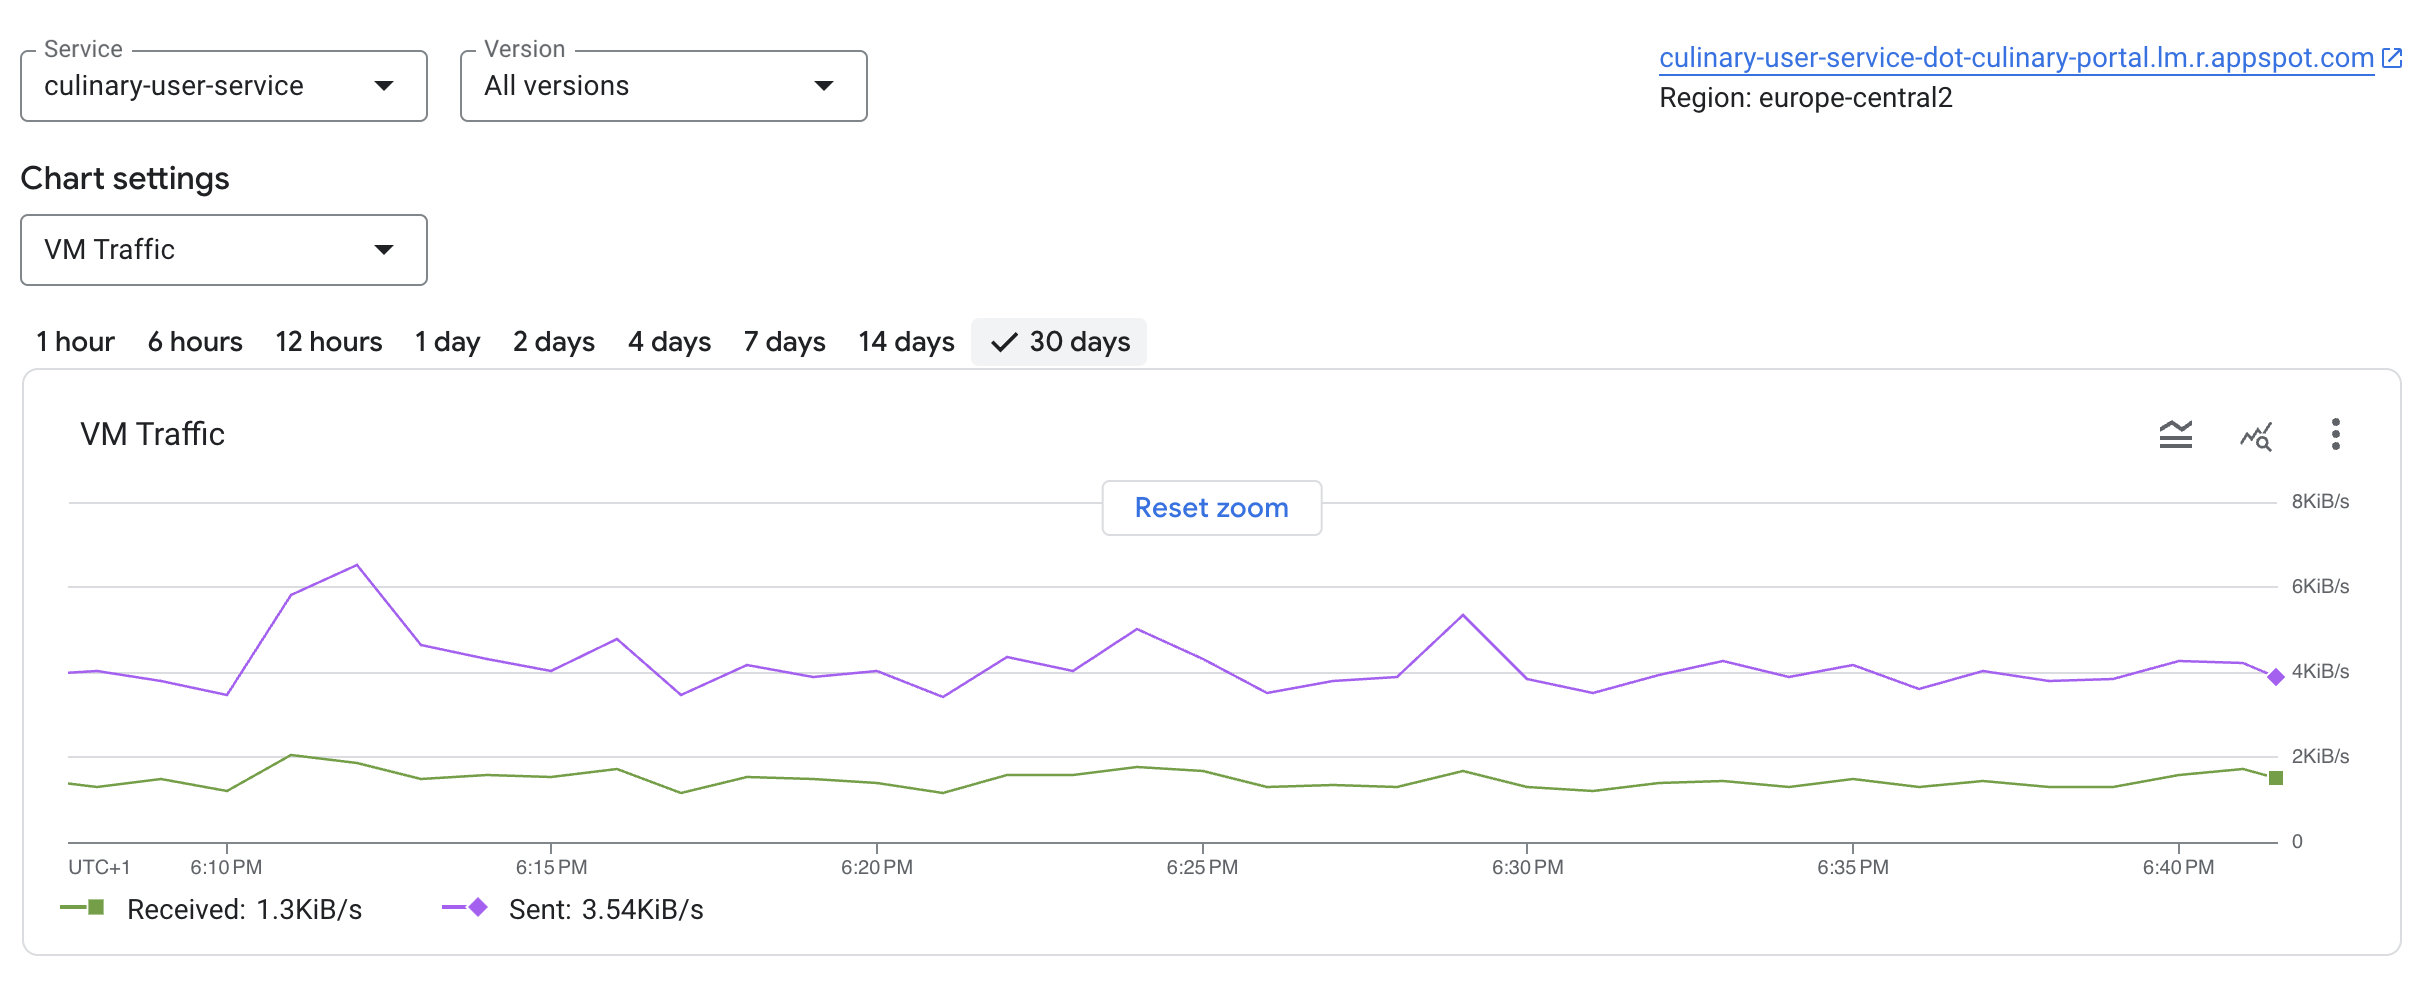
\includegraphics[width=1\textwidth]{images/GAE_monitoring.png}
    \caption{ GAE monitoring dashboars (culinary-user-service).}
    \label{GAE_monitoring}
\end{figure}

\subsection{Memorystore: Redis}\label{subsection:Memorystore: Redis}

Memorystore \cite{Memorystore} is a Google Cloud-managed Redis service, serves as the cloud-based version of the Redis database in our application architecture. Being a fully managed service meaning developer does not have to set up any machines, the management, patching, backup. Memorystore is easy to set up and maintain, eliminating much of the complexity typically associated with self-hosted Redis deployments. As a cloud-native solution, it uses Google Cloud’s infrastructure to deliver high-speed, low-latency data retrieval, making it an ideal choice for tasks such as caching and session management, which is crucial for us. One of the key advantages of using Memorystore is its high availability, ensuring that data is accessible even in the event of failures or maintenance. Furthermore, it provides exceptional scalability, enabling the system to grow alongside the application's needs. As the application scales, we do not have to worry about data migration or managing additional infrastructure. Memorystore allows us to simply scale up or out, ensuring continuous performance improvements without significant changes to the architecture. It also integrates well with the Spring framework through the Spring Data Redis library and Cloud GCP library, allowing for straightforward configuration and management and session handling within the application

\subsection{Cloud SQL: PostgreSQL}\label{subsection:Cloud SQL: PostgreSQL}

Cloud SQL \cite{Postgres} is a fully managed relational database service, is used in our application to host PostgreSQL, providing a reliable and scalable solution for managing structured data. Like Memorystore \ref{subsection:Memorystore: Redis}, Cloud SQL eliminates the complexity of database administration, offering automated backups, patching, and seamless scaling, which allows developers to focus on building features rather than maintaining infrastructure. The service is designed to deliver high availability and resilience, ensuring that data is accessible even in the event of failures or maintenance. Cloud SQL provides seamless integration with the Google Cloud ecosystem, ensuring that our PostgreSQL instance works efficiently with other services like Google App Engine. This integration ensures that as our application grows, we can scale the database with minimal effort and without worrying about migration or changing the system. The service also integrates well with the Spring framework, allowing developers to manage PostgreSQL connections through Spring Data JPA by adding connection details in application properties, as shown in Figure \ref{fig:postgres-connection}.

{
\begin{minted}[linenos, frame=single]{yaml}
spring:
  datasource:
    username: ${DB_USERNAME}
    password: ${DB_PASSWORD}
    driver-class-name: org.postgresql.Driver
  cloud:
    gcp:
      sql:
        enabled: true
        database-name: ${DB_NAME}
        instance-connection-name: ${DB_CONNECTION_NAME}
      credentials:
        encoded-key: ${GCP_SA_JSON} # for authenticating to GCP resource
\end{minted}
\captionof{figure}{application.yaml for Cloud SQL connection}
\label{fig:postgres-connection}
}

\subsection{Google Artifact Registry}\label{subsection:Google Artifact Registry}

Google Artifact Registry (GAR) \cite{GAR} is a fully managed service for storing and managing containerized application artifacts, such as Docker images. In our project, GAR is used to securely store Docker images for both the backend and frontend services in different folders shown in Figure \ref{GAR_folders}, ensuring that application artifacts are available for deployment. GAR integrates well with GAE Flex, simplifying the deployment process. It also supports versioning, making updates and rollbacks easier. To optimize costs, we have implemented a policy to remove old, unused images, reducing storage expenses while maintaining efficient artifact management within the Google Cloud environment.

 \begin{figure}[H]
    \centering
    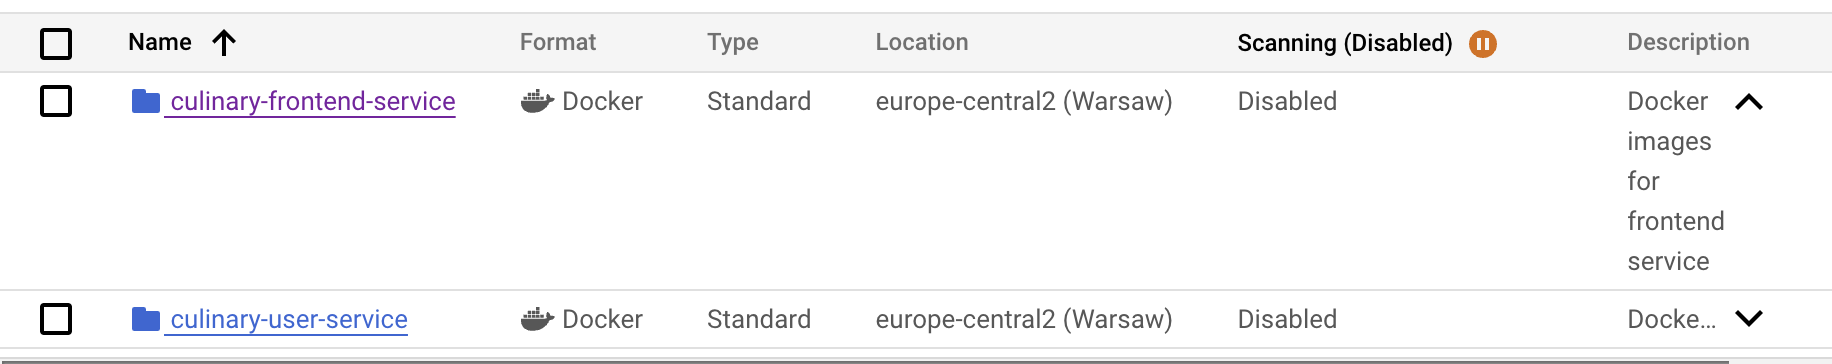
\includegraphics[width=1\textwidth]{images/gar-folders.png}
    \caption{ GAR repository for docker images.}
    \label{GAR_folders}
\end{figure}

\subsection{Google Service Accounts and Permissions}\label{subsection:Google Service Accounts and Permissions}

In a cloud environment, managing permissions and securing resources are critical aspects of application development and deployment. In the GCP project, we utilize Service Accounts combined with RBAC (Role-Based Access Control) to ensure secure and efficient access management across services and resources. Service accounts are special Google Cloud accounts designed for application and service interactions rather than human users. They play a central role in maintaining the principle of least privilege, ensuring each service or process has access only to the resources it needs.

When creating our solution, we used special accounts for separate functions aiming at reducing the potential threats in case of a security breach. All service accounts are scoped into specific RBAC roles and capabilities, which are necessary to be safe as much as possible in their operations. This organized strategy of levels of access, as well as access to resources, creates a stable environment for the more sensitive parts of the system.

For deployment purposes, we use a dedicated service account with permissions tailored for pushing Docker images to GAR and deploying applications to GAE. This account has roles like Artifact Registry Writer and App Engine Deployer assigned, ensuring that the CI/CD (Continuous Integration and Continuous Deployment) pipeline \ref{subsec:deployment-github-actions} can build, store, and deploy application containers securely without granting unnecessary access to other resources. The use of RBAC here helps limit what this service account can do, reducing the risk of accidental or malicious actions.

On the application side, the culinary-user-service (backend) uses a different service account to interact with Google Memorystore and Cloud SQL. This account is granted roles like Cloud Memorystore Redis User and Cloud SQL Client  to enable secure access to these resources. For development purposes, as developers, we have extensive access to the resources needed for efficient development and testing. However, full administrative control of the project is restricted to a single cloud Project Owner which is Kamil Dędza. This individual is the only one with comprehensive permissions, ensuring strict control over sensitive operations like project-wide configuration, billing, and roles management. This setup balances effective development flexibility with good security and management practices.

\subsection{Deployment with GitHub Actions}
\label{subsec:deployment-github-actions}

In modern software development, automation plays a crucial role in development processes and improving efficiency. CI/CD are essential practices for automating the building, testing, and deployment of applications. One effective way to implement CI/CD is through the use of GitHub Actions, a known tool that allows for the automation of workflows directly within GitHub repositories.

The integration of GitHub Actions with Google Cloud services facilitates the deployment of applications to GAE using Docker containers stored in GAR. This automation ensures that code changes are consistently tested, built, and deployed to the cloud environment without manual intervention of the developer, reducing space for human error and increasing the speed of project deliveries.

The workflow involves several key stages, including authenticating to Google Cloud, building and pushing Docker images, injecting necessary secrets into configuration files, and finally deploying the application to GAE. By leveraging GitHub Actions, developers can maintain an efficient and reliable CI/CD pipeline, ensuring that new features and updates are delivered seamlessly to the production environment. Workflow file for backend service is available on our \href{https://github.com/culinary-portal/culinary-user-service/blob/main/.github/workflows/build-deploy.yml}{github}.

Figure \ref{fig:ci_cd} provides a visual representation of the CI/CD pipeline process with GitHub Actions, outlining each step involved from code push to deployment.
\begin{figure}[H] % htbp specifies placement options (here, top, bottom, or page)
    \centering
    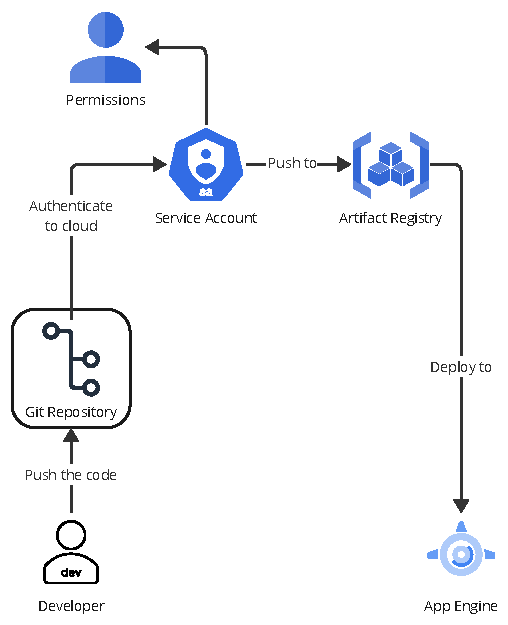
\includegraphics[width=0.6\textwidth]{meta/ci_cd_cropped.pdf}
    \caption{CI/CD with Github Actions (created by the Authors)}
    \label{fig:ci_cd}
\end{figure}
\subsection{Cloud Infrastructure Overview}

The system is designed for efficient communication between these services. The culinary-user-service (backend) communicates with Memorystore Redis for user session management and Cloud SQL Postgres for accessing business data. The frontend and backend services are integrated through APIs securely, allowing the frontend to fetch data and perform operations by interacting with the backend. This clear separation of logic between the frontend and backend makes the system more maintainable, and it allows both components to scale independently depending on usage demands. The overview of communication is presented on Figure \ref{fig:Current cloud infrastructure}.

\begin{figure}[H]
    \centering
    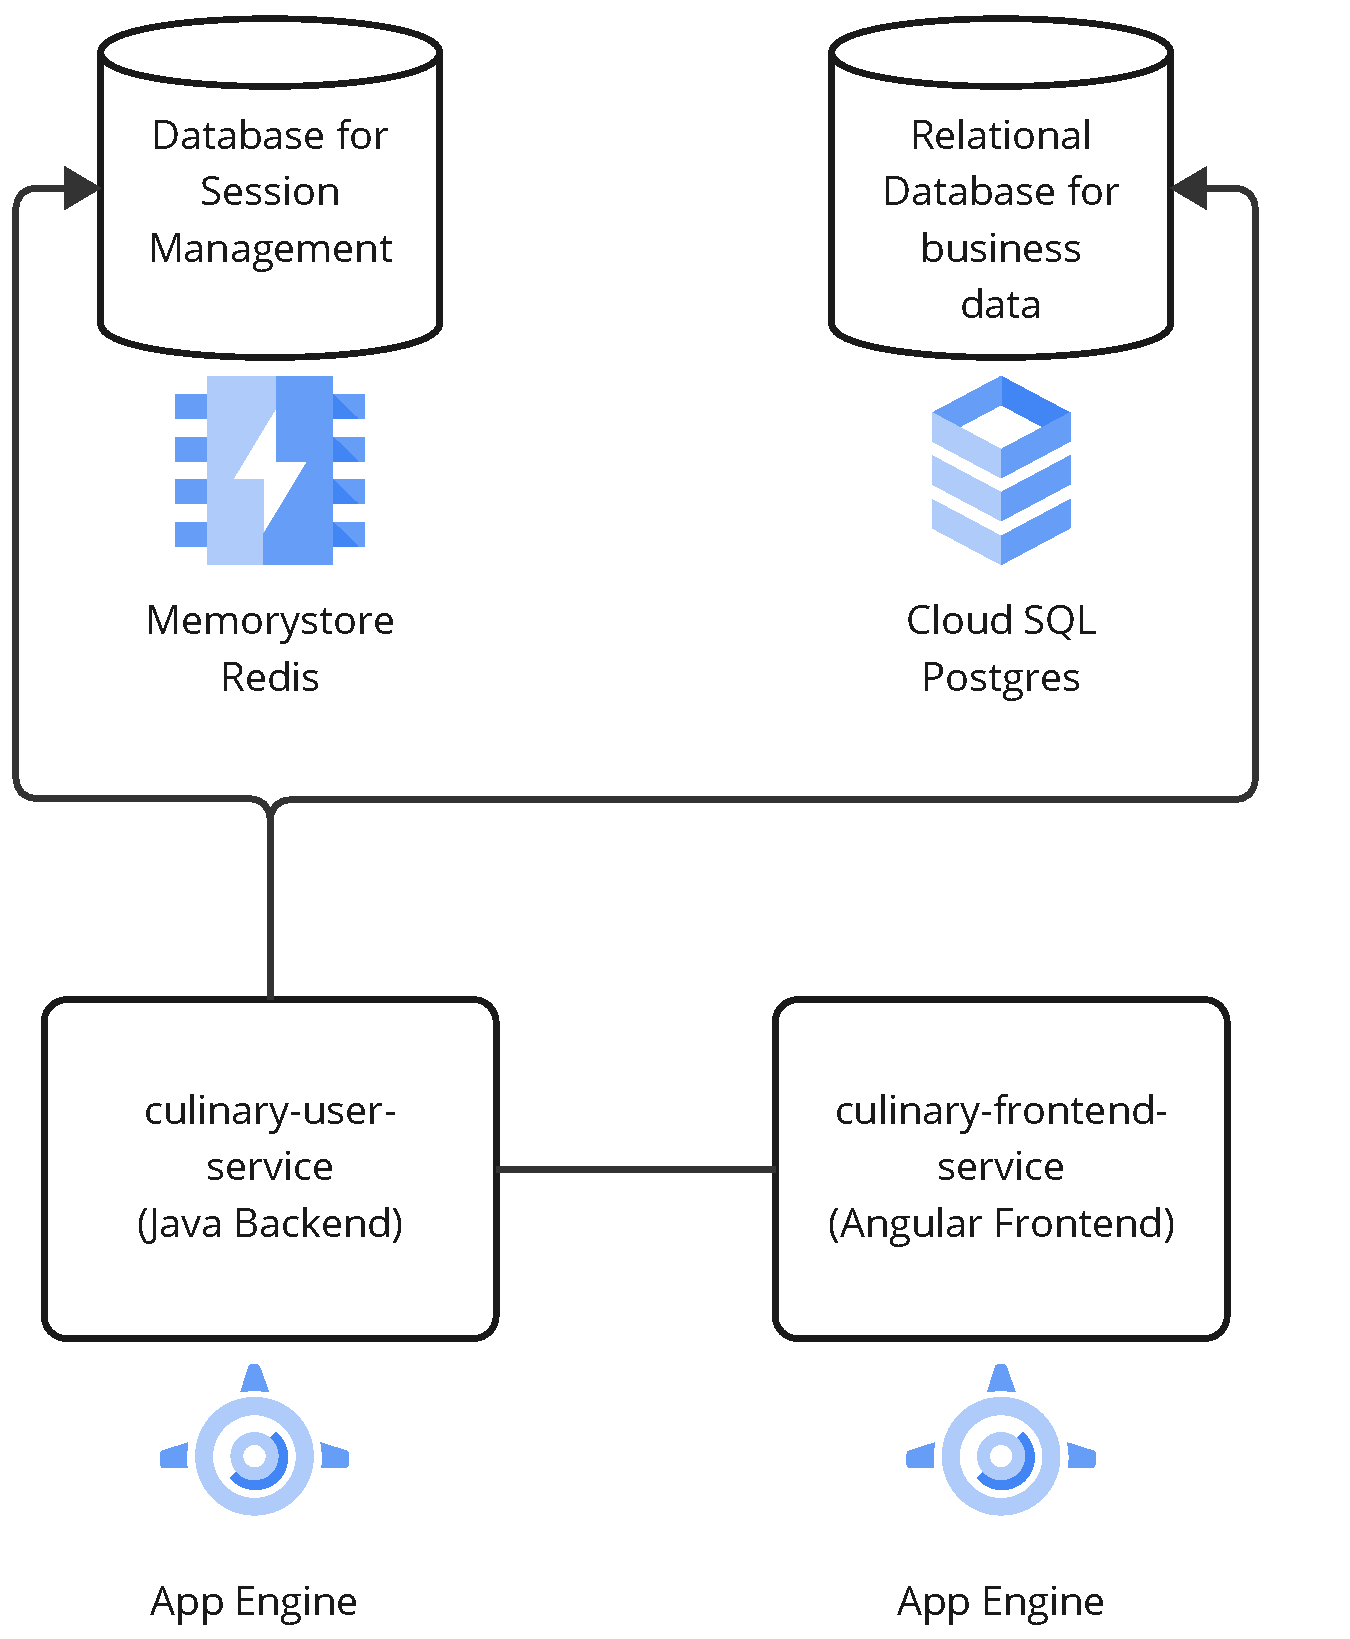
\includegraphics[width=0.6\textwidth]{meta/cloud_arch_cropped.pdf}
    \caption{Current cloud infrastructure (created by the Authors)}
    \label{fig:Current cloud infrastructure}
\end{figure}

The infrastructure is very scalable and resilient, using the capabilities for automatic scaling of Google App Engine to handle different loads, reducing hosting costs. Moreover, managed services like Memorystore (Redis) and Cloud SQL provide high availability and failovers, which ensure that the data is kept securely and remains available even in outages. This architecture is a good example of various cloud engineering practices such as microservices architecture, cloud-native design, and the use of managed services to reduce the complexity of the system.


